%! Author = rj
%! Date = 12/11/24

\documentclass{article}
\usepackage[utf8]{inputenc}
\usepackage{amssymb}
\usepackage{amsmath}
\usepackage{graphicx}
\usepackage[a4paper,margin=1in,footskip=0.25in]{geometry}
\usepackage[⟨options⟩]{fancyhdr}

\graphicspath{{Images/}}

\begin{document}
    \pagestyle{fancy}
    \fancyhead[LE, LO]{Richard Moser}
    \fancyhead[RE, RO]{01 December 2024}
    \fancyhead[CE, CO]{ASTR 691 PS5}

%    1. Stellar Structure – of the Earth! I. [17 pts]. Planets like the Earth are governed by some of the same structure
%    equations that we introduced for stellar interiors. Limit your answers below to two significant figures; the crude
%    model we’ll use below often isn’t even that accurate.
%    (a) Let’s make the simplest possible model – assume that the Earth has a constant density, ρ0. Given the
%    known mass and radius of the Earth, calculate ρ0. [2 pts]
%    (b) Assuming a constant density, calculate and plot the Earth’s enclosed mass, Menc(r), from 0 < r < R⊕.
%    What do you calculate for Menc(r = R⊕), i.e. for the total mass of the Earth (M⊕)? Explain how well
%    your answer compares to the true, measured mass of the Earth. [5 pts]
%    (c) Assuming a constant density, calculate and plot the Earth’s internal gravity field, g(r), for 0 < r < R⊕.
%    Explain how well your answer for g(r = R⊕) compares to the true, measured surface gravity at the surface
%    of the Earth. [5 pts]
%    (d) Assuming a constant density, calculate and plot the Earth’s internal pressure, P(r), for 0 < r < R⊕.
%    Calculate the pressure at the very center of the Earth, Pc = P(r = 0). [5 pts]
%    2. Stellar Structure – of the Earth! II. [24 pts]. For this problem, download the “Preliminary Reference Earth
%    Model” file from https://crossfield.ku.edu/files/preliminary_reference_earth_model.
%    csv. For all parts of this problem that involve calculations, be sure to explain your methods and/or show your
%    work. Note that you will need to do some simple numerical integration for this problem: this is best done using
%    your favorite programming language, but spreadsheet programs such as LibreOffice Calc can be made to do this
%    work in a pinch. (Limit numerical answers to three significant figures; I scraped the data file from a figure in a
%    paper, so the data values aren’t likely to be more precise than that.)
%    (a) Plot the Earth’s density profile ρ(r) (from the data file). Explain why you think the density profile has the
%    general shape that it does (don’t worry about explaining every little wiggle, but focus on the larger overall
%    features). [4 pts]
%    (b) (i) Calculate and plot the Earth’s enclosed mass, Menc(r), from 0 < r < R⊕. (ii) Describe and try to
%    explain the general, overall features shown in your plot. (iii) What do you calculate for Menc(r = R⊕),
%    i.e. for the total mass of the Earth (M⊕)? Explain how well your answer compares to the true, measured
%    mass of the Earth. [6 pts]
%    (c) Calculate and plot the Earth’s internal gravity field, g(r), for 0 < r < R⊕. The plot you get may surprise
%    you – it did me! Describe and try to explain the general, overall features shown in your plot. Explain how
%    well your answer for g(r = R⊕) compares to the true, measured surface gravity at the surface of the Earth.
%    [6 pts]
%    (d) Calculate and plot the Earth’s internal pressure, P(r), for 0 < r < R⊕. Give the central pressure, Pc, for
%    this model and describe how it compares to the central pressure you calculated in the previous problem. [6
%    pts]

    \textbf{1. Stellar Structure – of the Earth! I.}\\
    \textbf{(a)} Let’s make the simplest possible model – assume that the Earth has a constant density, $\rho_{0}$.
    Given the known mass and radius of the Earth, calculate $\rho_{0}$. \\
    \textbf{answer:} \\
%    \begin{equation}
%        \rho_{0} = \frac{M_{\oplus}}{\frac{4}{3}\pi R_{\oplus}^{3}} = 5.51 \times 10^{3} \text{ kg/m}^{3}
%    \end{equation}
    The mass of the Earth is $M_{\oplus} = 5.972 \times 10^{24} kg$ \\
    The radius of the Earth is $R_{\oplus} = 6.371 \times 10^{6} m$ \\
    The volume of the Earth is $V = \frac{4}{3}\pi R_{\oplus}^{3}$ \\
    The density of the Earth is $\rho_{0} = \frac{M_{\oplus}}{V}$. \\
%    $\rho_{0} = \frac{M_{\oplus}}{\frac{4}{3}\pi R_{\oplus}^{3}} = \frac{5.972 \times 10^{24} kg}{\frac{4}{3}\pi (6.371 \times 10^{6})^{3} m^{3}} = 5.52 \times 10^{3} kg/m^{3}$.
    $\rho_{0} = \frac{M_{\oplus}}{\frac{4}{3}\pi R_{\oplus}^{3}} = \frac{5.972 \times 10^{24} kg}{\frac{4}{3}\pi (6.371 \times 10^{6})^{3} m^{3}}$ \\
    \boxed{\rho_{0} = 5.52 \times 10^{3} kg/m^{3}} \\

    \textbf{(b)} Assuming a constant density, calculate and plot the Earth’s enclosed mass, $M_{enc}(r)$, from $0 < r < R_{\oplus}$.
    What do you calculate for $M_{enc}(r = R_{\oplus})$, i.e. for the total mass of the Earth ($M_{\oplus}$)? Explain how well
    your answer compares to the true, measured mass of the Earth. \\
    \textbf{answer:} \\
    $M_{enc}(<r) = \int_{0}^{r}dm = \int_{0}^{r}4\pi r^{2}\rho dr$ \\
    $M_{enc}(r) = \frac{4}{3}\pi r^{3}\rho_{0}$ for constant density $\rho_{0}$ \\
%    $M_{enc}(r = R_{\oplus}) = \frac{4}{3}\pi (6.371 \times 10^{6})^{3} 5.52 \times 10^{3} = 5.972 \times 10^{24} kg$ \\
    $M_{enc}(r = R_{\oplus}) = \frac{4}{3}\pi (6.371 \times 10^{6})^{3} 5.52 \times 10^{3}$ \\
    \boxed{M_{enc}(r = R_{\oplus}) = 5.972 \times 10^{24} kg} \\

    \textbf{(c)} Assuming a constant density, calculate and plot the Earth’s internal gravity field, $g(r)$, for $0 < r < R_{\oplus}$.
    Explain how well your answer for $g(r = R_{\oplus})$ compares to the true, measured surface gravity at the surface
    of the Earth. \\
    \textbf{answer:} \\
    See Figure 1.
    By using the constant value for $\rho$ calculated previously, the maximum (i.e. surface) value of gravity was
    9.82ms$^{-2}$ which is extremely close to the actual average surface gravity observed on Earth's surface. This is
    an overestimation of roughly 1\% which is surprisingly accurate.

    \begin{figure}[htp]
        \centering
        \includegraphics[width=5in]{PS5_1c.png}
        \caption{Earth's Internal Gravity Field}
        \label{Graph 1}
    \end{figure}

    \newpage
    \textbf{(d)} Assuming a constant density, calculate and plot the Earth’s internal pressure, $P(r)$, for $0 < r < R_{\oplus}$.
    Calculate the pressure at the very center of the Earth, $P_{c} = P(r = 0)$. \\
    \textbf{answer:} \\
    See Figure 2.
    $P(r) = \frac{GM_{enc}(r)\rho}{r}$ \\
%    (2/3) * np.pi * G * rho**2 * (R_earth**2 - r**2)
    $P(r) = \frac{2}{3}G \pi \rho_{0}^{2} (R_{\oplus}^2 - r^2)$ \\
    $P(r = 0) = \frac{2}{3}G \pi \rho_{0}^{2} (R_{\oplus}^{2})$ \\
    $P(r = 0) = \frac{2}{3} (6.67430 \cdot 10^{-11}) \pi (5.52 \cdot 10^{3})^{2} (6.371 \cdot 10^{6})^{2}$ \\
%    $P(r = 0) = 1.08 \cdot 10^{11} Pa$ \\
    \boxed{P(r = 0) \approx 1.73 \cot 10^{11} Pa} \\

    \begin{figure}[htp]
        \centering
        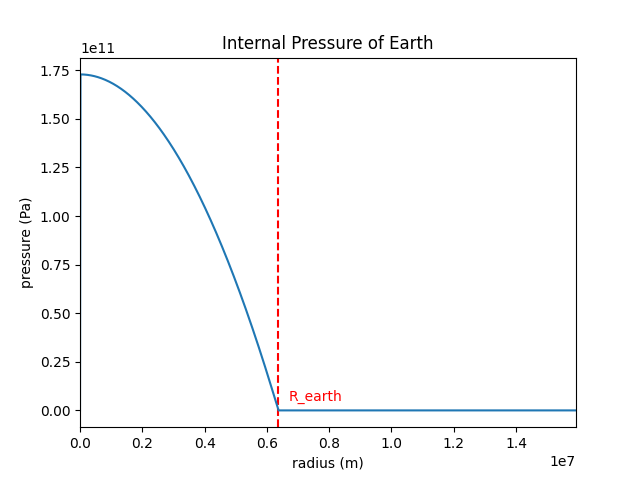
\includegraphics[width=5in]{PS5_1d.png}
        \caption{Earth's Internal Pressure}
        \label{Graph 2}
    \end{figure}

    $\break$
    \newpage
    \textbf{2. Stellar Structure – of the Earth! II.}\\
    \textbf{(a)} Plot the Earth’s density profile $\rho(r)$ (from the data file). Explain why you think the density profile has the general shape that it does (don’t worry about explaining every little wiggle, but focus on the larger overall features). \\
    \textbf{answer:} \\
    See Figure 3.
    The density profile doesn't follow one smooth curve but it looks like it has a few discrete layers in which they have somewhat consistent density profiles. These likely correspond to the actual layers of the Earth's interior and the radii where the profile shifts abruptly are probably the radii at which the Earth's layers transition from one to the next. The difference in the shape of the curve from one layer to the next is probably due to the different materials which make up the layers and their respective densities.

    \begin{figure}[htp]
        \centering
        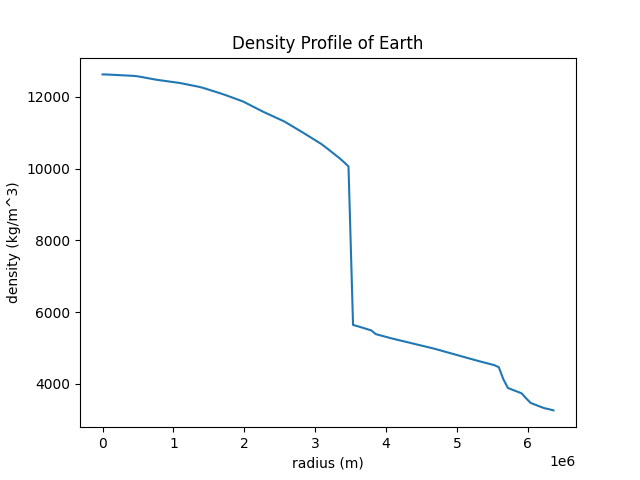
\includegraphics[width=5in]{PS5_2a.png}
        \caption{Earth's Density Profile}
        \label{Graph 3}
    \end{figure}

    \newpage
    \textbf{(b)} (i) Calculate and plot the Earth’s enclosed mass, $M_{enc}(r)$, from $0 < r < R_{\oplus}$. (ii) Describe and try to explain the general, overall features shown in your plot. (iii) What do you calculate for $M_{enc}(r = R_{\oplus})$, i.e. for the total mass of the Earth ($M_{\oplus}$)? Explain how well your answer compares to the true, measured mass of the Earth. \\
    \textbf{answer:} \\
    See Figure 4.
    The plot shows an exponential increase in mass up until about 3500 km where it resets to a lower slope before climbing again. This corresponds to the significant drop in density and likely a transition between two very different layers within the Earth. The total mass of the Earth is calculated to be $6.05 \times 10^{24}$ kg which is very close to the actual mass of the Earth, around $5.97 \times 10^{24}$ kg.

    \begin{figure}[htp]
        \centering
        \includegraphics[width=5in]{PS5_2b.png}
        \caption{Earth's Enclosed Mass}
        \label{Graph 4}
    \end{figure}

    \newpage
    \textbf{(c)} Calculate and plot the Earth’s internal gravity field, $g(r)$, for $0 < r < R_{\oplus}$. The plot you get may surprise you – it did me! Describe and try to explain the general, overall features shown in your plot. Explain how well your answer for $g(r = R_{\oplus})$ compares to the true, measured surface gravity at the surface of the Earth. \\
    \textbf{answer:} \\
    See Figure 5.
    Here again we see that 3500km marks an important transition in the Earth's interior. Up to this radius, internal gravity is increasing and then begins to drop off, though there seems to be a flattening nearer to the surface. It seems clear that the denser layers drive the steep rise in gravity but the drop off and flattening was unexpected. I suspect that the initial drop is due to the sudden drop in density with increasing radius, but and that the flattening is due to the much flatter density profile nearer to the surface.This does estimate the surface gravity to be 9.97ms$^{-2}$  which is a slight overestimation, but within a few percent of the true value.

    \begin{figure}[htp]
        \centering
        \includegraphics[width=5in]{PS5_2c.png}
        \caption{Earth's Internal Gravity Field}
        \label{Graph 5}
    \end{figure}

    \newpage
    \textbf{(d)} Calculate and plot the Earth’s internal pressure, $P(r)$, for $0 < r < R_{\oplus}$. Give the central pressure, $P_{c}$, for this model and describe how it compares to the central pressure you calculated in the previous problem. \\
    \textbf{answer:} \\
    See Figure 6.
    The pressure profile shows a somewhat similar overall shape to the density profile with much smoother transitions between layers. The central pressure is calculated to be about $3.83 \times 10^{11}$ Pa which is about 2.2 times the central pressure calculated in the previous problem. This is likely due to the more complex density profile which is not constant and has a few discrete layers.

    \begin{figure}[htp]
        \centering
        \includegraphics[width=5in]{PS5_2d.png}
        \caption{Earth's Internal Pressure}
        \label{Graph 6}
    \end{figure}



    $\break$

    $\break$
\end{document}